\setchapterpreamble[u]{\margintoc}
\chapter{The Regression Theory of Everything}
\labch{intro}

\textit{"AI Scientists disagree as to whether these language networks possess true knowledge or are just mimicking humans by remembering the statistics of millions of words. I don't believe any kind of deep learning network will achieve the goal of AGI [Artificial General Intelligence] if the network doesn't model the world the way the brain does. Deep learning networks work well, but not because they solved the knowledge representation problem. They work well because they avoided it completely, relying on statistics and lots of data instead. How deep learning networks work is clever, their performance impressive, and they are commercially valuable. I am only pointing out that they don't possess knowledge and, therefore, are not on the path to having the ability of a five-year-old child."} Jeff Hawkins, 2022 \cite{hawkins2022}

\section{Let's Avoid Knowledge Representation!}

The knowledge representation problem in AI is the challenge of how to formally represent knowledge in a way that a computer can understand and reason about. This typically involves creating a set of symbols, rules, and structures that can be used to represent concepts, relationships, and other types of information. The goal is to create a representation that is both expressive enough to capture all relevant aspects of the domain, and computationally tractable enough to allow for efficient reasoning and inference. There are many different approaches to knowledge representation, including logic-based, semantic networks, frames, and ontologies, each with their own strengths and weaknesses.

Deep learning techniques handle knowledge representation differently than traditional symbolic AI methods. Unlike symbolic AI, which relies on explicit and hand-coded representations of knowledge, deep learning techniques learn to represent knowledge implicitly through the use of neural networks.


\begin{marginfigure}[-5.5cm]
        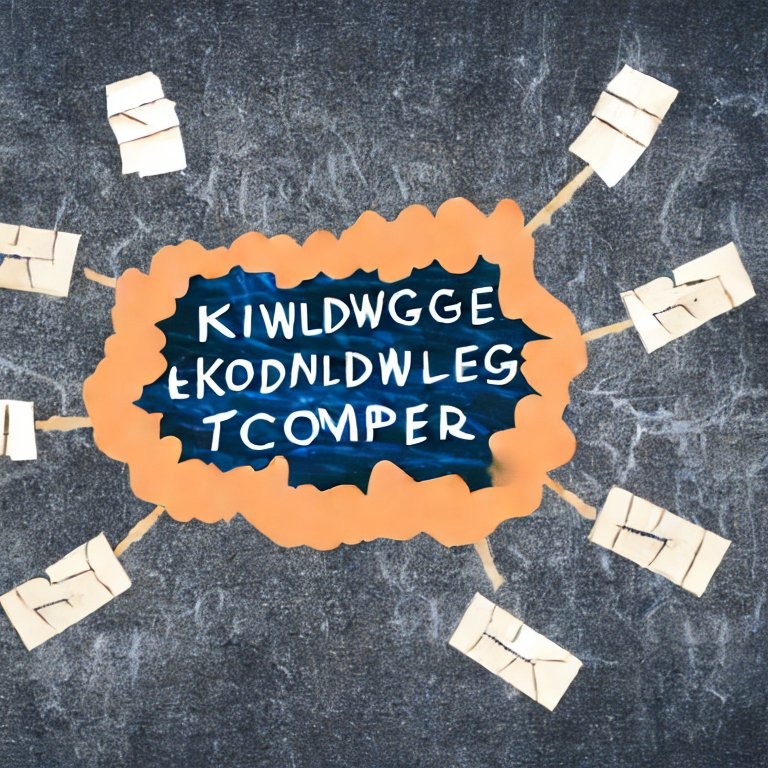
\includegraphics{knowledge}
        \caption{"mdjrny-v4 a disembodied computer being force-fed data like a duck looking somewhat like a sci-fi character 8k" made with OpenJourney}
        \labfig{marginknowledge}
\end{marginfigure}


In deep learning, knowledge is represented in the form of the weights of the neural network. These weights are learned through training on a large dataset and they capture the underlying relationships and patterns in the data. The neural network can then use these learned weights to make predictions, classifications or generate new data.

Deep learning models can handle large and complex datasets, and can automatically extract features from the data without the need for manual feature engineering. This makes them particularly well-suited for tasks such as image and speech recognition, natural language processing, and other areas where large amounts of data are available. However, they are not as good at explicating how they arrived at a decision, which can be a disadvantage.

In summary, deep learning techniques handle knowledge representation by learning the underlying patterns and relationships in the data through the use of neural networks, which can then be used for prediction, classification, and generation tasks.

\section{A Simple Neural Network is also a Linear Regression}

A neural network can be mathematically equivalent to a regression or a decision tree under certain conditions.

A neural network is a machine learning model composed of layers of interconnected artificial neurons, which are designed to process and analyze data. They can be used for a wide range of tasks, such as image and speech recognition, natural language processing, and prediction.

\begin{marginfigure}[-5.5cm]
	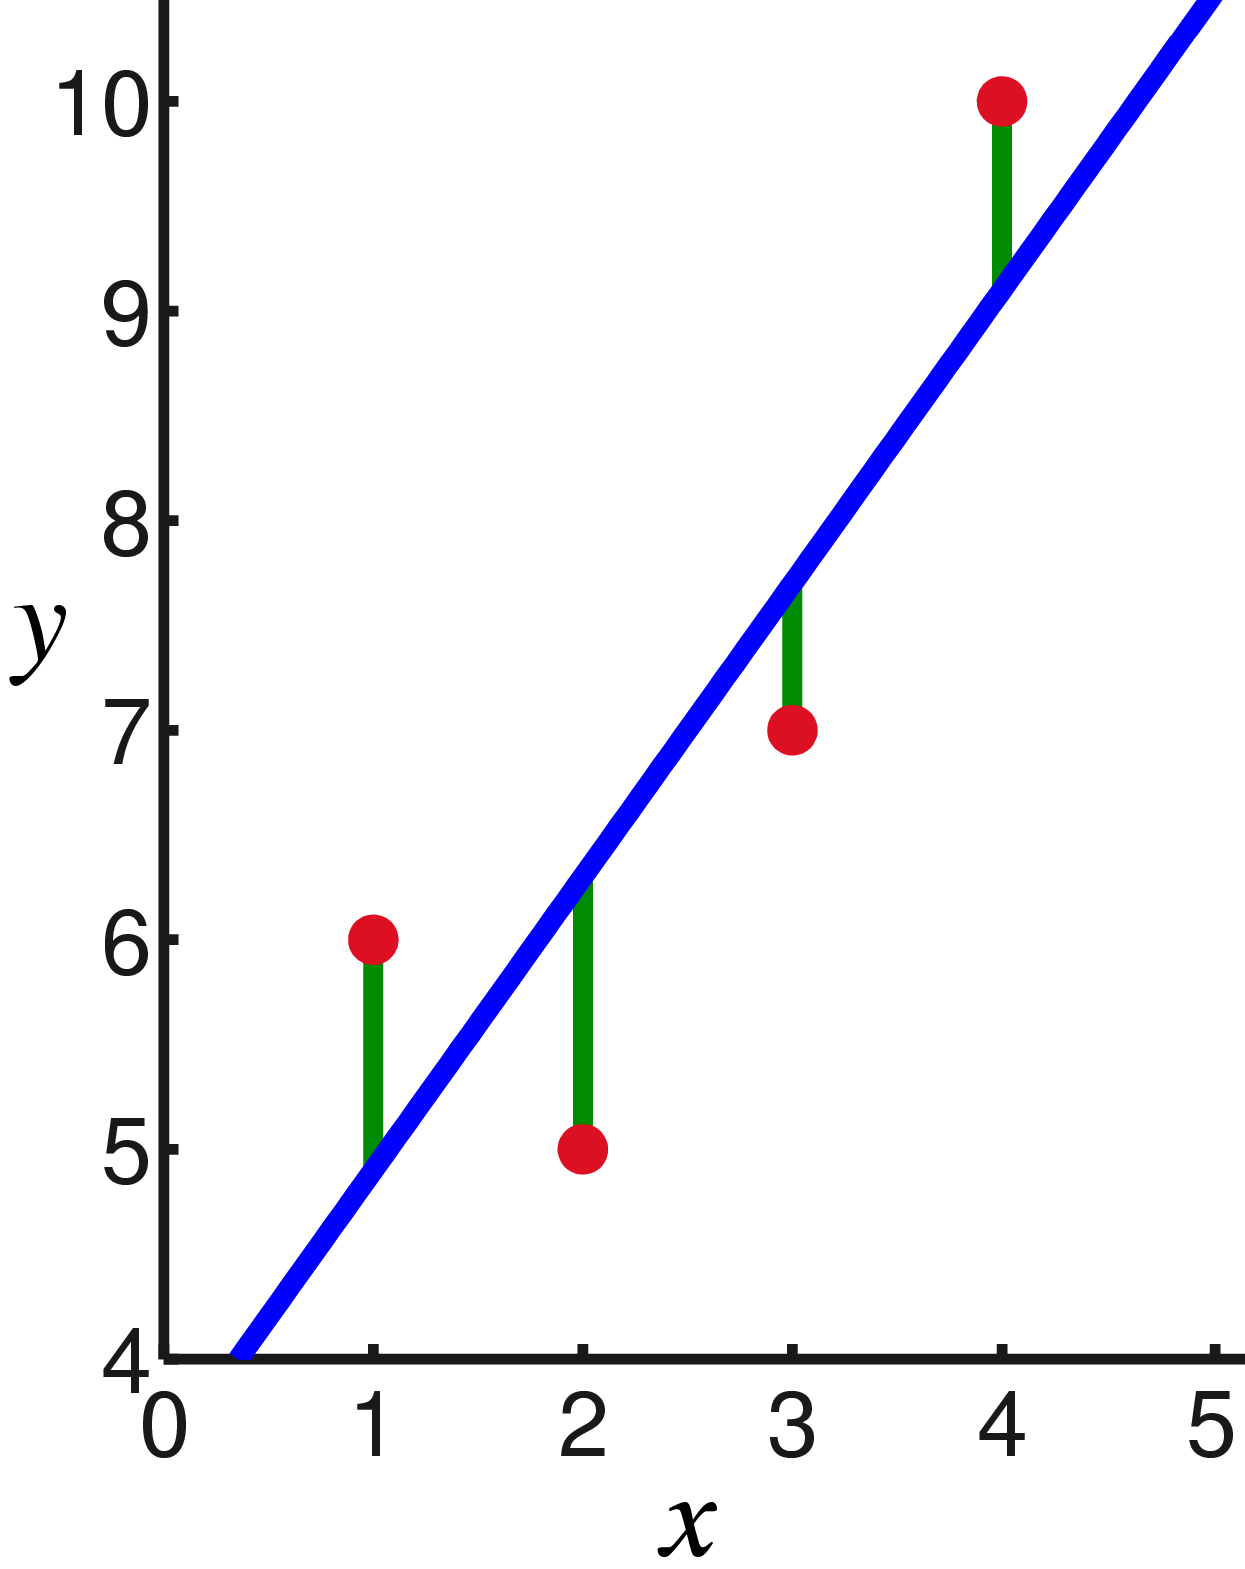
\includegraphics{OLSregression}
        \caption{A simple linear regression, the red points are the training data, and the blue line is the regression line. If you don't understand this please read \url{https://en.wikipedia.org/wiki/Regression_analysis}}
        \labfig{olsregression}
\end{marginfigure}


A regression is a statistical method used to predict a continuous variable based on one or more input features. A linear regression, for example, is a simple neural network with one input layer, one output layer and no hidden layers. In this case, the weights of the network are the coefficients of the linear equation and the network is equivalent to a linear regression model.

A decision tree is a tree-based model used for classification and prediction tasks. It consists of a series of if-then rules that are used to make decisions based on the input data. A neural network with one input layer, one output layer and one hidden layer with the ReLU activation \sidenote{Neurons in a neural network can have different activation functions, if you don't know what it is and don't want to read about it on wikipedia, that's OK. \url{https://en.wikipedia.org/wiki/Activation\_function}} function is equivalent to a decision tree. This is because the ReLU activation function allows the network to implement a piecewise linear function which can represent the decision boundaries of a decision tree.

In summary, under certain conditions, a neural network can be mathematically equivalent to a linear regression or a decision tree. These conditions include having one input and one output layers, and having a specific activation function in the case of a decision tree.\sidecite{Aytekin}

\section{Dummy Variables for Dummies (Wonkish)} 

Chapter Summary: It's all numbers, man. Machine learning techniques require that we turn everything (images, text, sound) into numbers and shove them into the model in the same way we use dummy variables in a simple regression. If you are satisfied with this, please skip this section. If you would like to learn a bit about the details and see some code examples, please keep reading. This section is necessarily technical, but should be approachable for anyone who has taken a college statistics class. \sidenote{Thanks to Paul Krugman for popularizing (to me at least) the \textit{wonkish} classifier, I just mean it's a little nerdy. But it's important.} 



Dummy variables are used in regression analysis to include categorical variables in a model. Categorical variables are variables that take on a finite number of distinct values, such as "red", "green", "blue" or "yes", "no". Since these variables cannot be directly included in a regression model, as they are not numerical, they need to be transformed into numerical variables.

The process of creating dummy variables is also known as one-hot encoding. It involves creating a new binary variable for each category of the original variable. For example, if you have a categorical variable "color" with three categories: "red", "green", "blue", you would create three binary variables: "color\_red", "color\_green", "color\_blue". Each binary variable would take a value of 1 if the original variable is equal to the category, and 0 otherwise.

When using dummy variables in a regression, it is important to remember to include only n-1 binary variables, where n is the number of categories in the original variable. This is because including all n binary variables would result in perfect multicollinearity, which is when two or more independent variables are perfectly correlated. One of the binary variables can be dropped to avoid this problem.

Dummy variables are used in regression analysis to include categorical variables in a model. The process of creating dummy variables involves creating a new binary variable for each category of the original variable and one-hot encoding it. It is important to remember to include only n-1 binary variables, to avoid perfect multicollinearity.



\begin{marginlisting}[-0.5cm]
\caption{Mapping text to numbers.}
\vspace{0.2cm}
\begin{lstlisting}[language=Python,style=kaolstplain]
 'movies': 99,
 'after': 100,
 'think': 101,
 'characters': 102,
 'watch': 103,
 'two': 104,
 'films': 105,
 'character': 106,
 'seen': 107,
 'many': 108,
 'being': 109
\end{lstlisting}
\end{marginlisting}


The creation of dummy variables in a regression is analogous to preprocessing image, text and other data for a neural network for deep learning. This preprocessing is important  as it ensures that the data is in a format that can be easily understood and processed by the network. The preprocessing steps for numbers, text, and images are slightly different.

For numbers:
\begin{itemize}
	\item Normalization: It is common to normalize the input data by scaling it to have a mean of 0 and a standard deviation of 1. This helps to ensure that all input features have similar scales and prevents any one feature from dominating the network's computations.
	\item Imputation: Handling missing data is important, as it can negatively impact the model's performance. Common imputation techniques include replacing missing values with the mean, median, or mode of the feature.
\end{itemize}

For text:

\begin{itemize}
	\item Tokenization: Text data must first be converted into a numerical format that can be understood by the network. This is typically done by tokenizing the text into individual words or n-grams and then encoding them as integers or real-valued vectors. A one-hot encoding exactly like the dummy variable method used in regression is also frequently used. \sidenote{Sometimes text is just mapped to a number! Shocking, but it works. See how it is taught in the TensorFlow tutorials \url{https://www.tensorflow.org/text/guide/word\_embeddings}} \sidenote{GPT-3 uses byte-level Byte Pair Encoding (BPE) tokenization and has a vocabulary size of 50,257.}
	\item Stop-words removal: The most common words in any language like "a", "an", "the", etc. that do not contain much meaning are called stop-words, they are often removed to reduce the dimensionality of the data.
	\item Stemming/Lemmatization: Words that have the same meaning can be stemmed or lemmatized to reduce the vocabulary size and increase the chances of generalization.
	\item Vocabulary Size: Each model must choose a vocabulary size or the maximum number of tokens that it will analyze. This may cause misspellings, slang or typos to be discarded in analysis.
\end{itemize}

For images:
    
\begin{itemize}
	\item Converting to RGB or Greyscale: Each image is analyzed by its pixel color value, every point on an image will either have 3 color values (red, green, blue) or one single value (on a white/black scale) if the image is analyzed in greyscale.
	\item Convolutions\sidenote{If you would prefer a visualization of a neural network check out this excellent video by Dennis Dmitriev \url{https://www.youtube.com/watch?v=3JQ3hYko51Y}.}: Pixel values are analyzed in groups that are defined by the model, since individual pixel values are only colors (or greyness) they must be combined together by the model to detect patterns like faces and stop signs. The method of convolution is defined by the model itself.
	\item Resizing: neural network can only accept images of a fixed size, so resizing the image to match the network's requirements is important.
	\item Normalization: It is common to normalize the pixel values to be in the range of 0-1 or -1 to 1. This will help the model converge faster.
	\item Data Augmentation: To increase the amount of data and prevent overfitting, common data augmentation techniques such as flipping, rotation, and cropping can be applied to the images.
\end{itemize}

In summary, preprocessing is an important step in training a neural network, as it ensures that the data is in a format that can be easily understood and processed by the network. The preprocessing steps for numbers, text, and images involve normalization, imputation, tokenization, stop-words removal, stemming/lemmatization, resizing and data augmentation.

\section{Try That Again With 33,640,010 Parameters}

In the first section of this chapter we introduced the idea that a simple neural network is mathematically equivalent to a regression. This is true and a useful way to think about neural networks and deep learning. \sidenote{\begin{equation}y=Wx+b\end{equation} There's your simple formula for a single-cell neural network and regression, in practice we'll change $W$, $x$ and $b$ to matrices and introduce nonlinear activation function $f$ so, \begin{equation}y=f(Wx+b)\end{equation} if you please. If equations scare you, don't worry about it for now.} 

In practice, neural networks frequently trained with millions of parameters. Here is an example of the trainable parameters of a simple image classifier. This example is a dense neural network to classify handwritten digits, and is not yet as sophisticated as the one used by Yann LeCun and company in the 1990s

In these next few examples, don't worry if you don't understand the layer types or know what batch nomalization means. The point I would like to make is that neural networks are often created with millions of trainable parameters, once you agree with me regarding this point we will discuss the implications of this in more depth.

\begin{lstlisting}[style=kaolstplain,linewidth=1.5\textwidth]
_________________________________________________________________
Layer (type)                 Output Shape              Param #   
=================================================================
dense (Dense)                (None, 64)                50240     
_________________________________________________________________
batch_normalization (BatchNo (None, 64)                256       
_________________________________________________________________
dense_1 (Dense)              (None, 64)                4160      
_________________________________________________________________
batch_normalization_1 (Batch (None, 64)                256       
_________________________________________________________________
dense_2 (Dense)              (None, 64)                4160      
_________________________________________________________________
batch_normalization_2 (Batch (None, 64)                256       
_________________________________________________________________
dropout (Dropout)            (None, 64)                0         
_________________________________________________________________
dense_3 (Dense)              (None, 10)                650       
=================================================================
Total params: 59,978
Trainable params: 59,594
Non-trainable params: 384
_________________________________________________________________
\end{lstlisting}

\begin{marginfigure}[-5.5cm]
        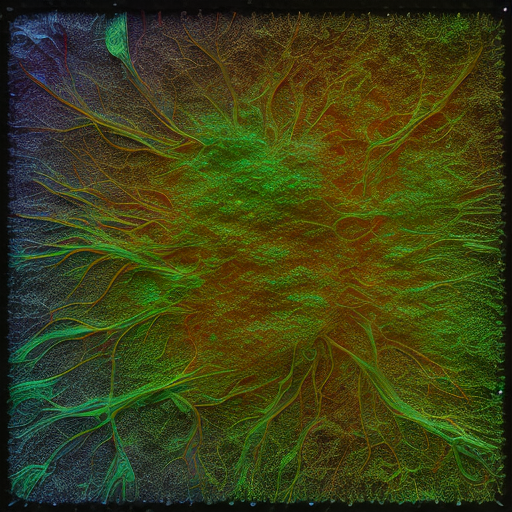
\includegraphics{greenneuron}
        \caption{"mdjrny-v4 layers and layers of neurons looking like a gooey lasagna, but the data has green blood 8k" made with OpenJourney}
        \labfig{marginneuron}
\end{marginfigure}

59,594 parameters! That's not too bad for a simple neural network, but in practice the networks often get even bigger. Here is a \textit{real} example that will make your brain a little hot.

\begin{lstlisting}[style=kaolstplain,linewidth=1.5\textwidth]
Layer (type)                 Output Shape              Param #   
=================================================================
conv2d (Conv2D)              (None, 28, 28, 64)        640       
_________________________________________________________________
conv2d_1 (Conv2D)            (None, 28, 28, 64)        36928     
_________________________________________________________________
max_pooling2d (MaxPooling2D) (None, 14, 14, 64)        0         
_________________________________________________________________
batch_normalization (BatchNo (None, 14, 14, 64)        256       
_________________________________________________________________
conv2d_2 (Conv2D)            (None, 14, 14, 128)       73856     
_________________________________________________________________
conv2d_3 (Conv2D)            (None, 14, 14, 128)       147584    
_________________________________________________________________
max_pooling2d_1 (MaxPooling2 (None, 7, 7, 128)         0         
_________________________________________________________________
batch_normalization_1 (Batch (None, 7, 7, 128)         512       
_________________________________________________________________
conv2d_4 (Conv2D)            (None, 7, 7, 256)         295168    
_________________________________________________________________
conv2d_5 (Conv2D)            (None, 7, 7, 256)         590080    
_________________________________________________________________
conv2d_6 (Conv2D)            (None, 7, 7, 256)         590080    
_________________________________________________________________
max_pooling2d_2 (MaxPooling2 (None, 3, 3, 256)         0         
_________________________________________________________________
batch_normalization_2 (Batch (None, 3, 3, 256)         1024      
_________________________________________________________________
conv2d_7 (Conv2D)            (None, 3, 3, 512)         1180160   
_________________________________________________________________
conv2d_8 (Conv2D)            (None, 3, 3, 512)         2359808   
_________________________________________________________________
conv2d_9 (Conv2D)            (None, 3, 3, 512)         2359808   
_________________________________________________________________
max_pooling2d_3 (MaxPooling2 (None, 2, 2, 512)         0         
_________________________________________________________________
batch_normalization_3 (Batch (None, 2, 2, 512)         2048      
_________________________________________________________________
conv2d_10 (Conv2D)           (None, 2, 2, 512)         2359808   
_________________________________________________________________
conv2d_11 (Conv2D)           (None, 2, 2, 512)         2359808   
_________________________________________________________________
conv2d_12 (Conv2D)           (None, 2, 2, 512)         2359808   
_________________________________________________________________
max_pooling2d_4 (MaxPooling2 (None, 1, 1, 512)         0         
_________________________________________________________________
batch_normalization_4 (Batch (None, 1, 1, 512)         2048      
_________________________________________________________________
flatten (Flatten)            (None, 512)               0         
_________________________________________________________________
dense (Dense)                (None, 4096)              2101248   
_________________________________________________________________
dropout (Dropout)            (None, 4096)              0         
_________________________________________________________________
dense_1 (Dense)              (None, 4096)              16781312  
_________________________________________________________________
dropout_1 (Dropout)          (None, 4096)              0         
_________________________________________________________________
dense_2 (Dense)              (None, 10)                40970     
=================================================================
Total params: 33,642,954
Trainable params: 33,640,010
Non-trainable params: 2,944
_________________________________________________________________
\end{lstlisting}

When a neural network has millions of trainable parameters and deep layers of neurons\sidenote{In case you are wondering, the human brain has about 86 billion neurons that do the "thinking". Physical neurons are more complicated than the neurons used in deep learning and have supporting structures like astrocytes that do some computation as well. \url{https://en.wikipedia.org/wiki/Astrocyte}}, it can be difficult to explain to a human what each of those parameters represents or how they contribute to the overall function of the network. This is because the interactions between the different layers and neurons can be complex and non-linear, making it challenging to understand the specific role of each parameter. The parameters  model complex interactions between the inputs, making it difficult to understand their specific function. Furthermore, in deep neural networks, the high number of layers can lead to high level of abstraction, meaning that the individual neurons and their weights have little interpretability.

When a neural network has millions of interacting parameters, it can lead to mathematical chaos \sidenote{Mathematical chaos is a real thing, it refers to the behavior of certain dynamic systems that are highly sensitive to initial conditions. This sensitivity leads to seemingly random and unpredictable behavior, even though the underlying equations governing the system are deterministic (meaning they are transparent and known to us). \url{https://en.wikipedia.org/wiki/Chaos_theory} }, which is a phenomenon where small changes in the initial conditions of the network can lead to vastly different outputs. This is because the interactions between the large number of parameters can create non-linear relationships that are sensitive to small changes. This can make it difficult to predict the behavior of the network, as small changes in the input or the parameters can lead to unexpected and seemingly random outputs.\sidenote{Chaotic outputs in a large deterministic system are OK in many domains, and there are controls that can be put in place to keep AI "safe" but deep learning by itself will not produce those controls.}

\section{Multicolinearity and the End of Science}

Data science is a horrible term because it implies that data scientists are scientists and that the work they do is scientific when in reality data scientists are not scientists and the work they do is not scientific. Data scientists use mathematics, statistics, and computer science to analyze data, but it is not scientific in the traditional sense. Data scientists do not use the scientific method and do not conduct experiments or develop theories. Data science is more akin to engineering or data analytics than actual scientific research.

The main goal of a scientist is to gain knowledge and understanding of the natural world through research, experimentation, and data analysis. Scientists make models of the world to test and explain. So-called data scientists make models too but a model with layers of interacting parameters, trained under chaotic conditions is almost impossible to explain. Multicolinearity\sidenote{"Multicolinearity is when two or more variables in a study are closely related to each other. Think of it like dating: imagine you are trying to figure out what makes someone a good partner. You might look at things like how much they make, how attractive they are, and how kind they are. But, these things are all related to each other. For example, attractive people might make more money, and kind people might be more attractive. So, it's hard to know which one is really important for being a good partner, because they are all related. That's like multicolinearity in a study." By ChatGPT given the prompt "explain multicolinearity to a teenager using a dating example"} is just one issue, but deep learning techniques are practically incompatible with the scientific method. With deep learning methods it can be difficult to determine which variable had the most impact on the outcome of the model. Coefficients of the model to be unstable and unreliable, which can make it difficult to explain the model in a meaningful way. 

Explaining the inner-workings of a neural network with millions of interacting parameters is difficult for many reasons. Most of the complexity is due to the number of parameters, which can make it difficult to understand how the model works and why it makes certain decisions. The interactions between the parameters are often non-linear and can be difficult to understand, as the model can be sensitive to small changes in the parameters, which is the definition of mathematical chaos. This can make it difficult to explain why the model is making certain decisions, as the interactions between the parameters are not always clear.

\section{Let's Test Some Random Inputs! Feature Importance and Explainability}

With a huge complex system of neurons that combine inputs in novel ways, it becomes vary hard to understand which inputs are the most important for the system as a whole. To better understand deep learning models, data scientists use randomized or averaged inputs to a model to test the feature importance of a deep learning neural network. This type of testing is done to determine which features are most influential in the overall output of the network. This is done by randomly or averaging the input values for each feature and then running the model to see how the output is affected. For example, if a neural network is used to detect objects in an image, the data scientist may randomize the color of the objects to see how the model’s accuracy is affected. If the accuracy drops significantly, they can infer that color is an important feature in the network.

Randomized or averaged inputs to a model can also be used to determine if a particular feature is necessary for the network to function correctly. For example, if the output of the network is not as accurate when a particular feature is randomized or averaged, then the data scientist can infer that this feature is important for the network’s performance. By using this method, data scientists can gain insights into which features are important and which can be removed from the model to improve performance.

\section{The Universal Machine Learning Workflow}

The Universal Machine Learning Workflow\sidecite{chollet2022} is an important chapter in a technical guide for data scientists  by the author of the most popular machine learning framework in the world\sidenote{It's called TensorFlow and was one of the most popular and "Most Loved" Technologies of 2022 \url{https://survey.stackoverflow.co/2022/\#most-popular-technologies-misc-tech}} that outlines the \textit{Universal} workflow for machine learning projects. I think this chapter should be understood by everyone using, investing in and creating machine learning models. 

Before Chollet gets into the details of model building, he chooses to begin with a note on ethics: 

\textit{"You may sometimes be offered ethically dubious projects, such as “building an AI that rates the trustworthiness of someone from a picture of their face.” First of all, the validity of the project is in doubt: it isn’t clear why trustworthiness would be reflected on someone’s face. Second, such a task opens the door to all kinds of ethical problems. Collecting a dataset for this task would amount to recording the biases and prejudices of the people who label the pictures. The models you would train on such data would merely encode these same biases into a black-box algorithm that would give them a thin veneer of legitimacy. In a largely tech-illiterate society like ours, “the AI algorithm said this person cannot be trusted” strangely appears to carry more weight and objectivity than “John Smith said this person cannot be trusted,” despite the former being a learned approximation of the latter. Your model would be laundering and operationalizing at scale the worst aspects of human judgement, with negative effects on the lives of real people.}

\begin{marginfigure}[-5.5cm]
        
\includegraphics{trustworthysd}
        \caption{"the face of a trustworthy person" made with Stable Diffusion 2.1. (Hey, it's a white lady!)}
        \labfig{trustworthysd}
\end{marginfigure}

\textit{Technology is never neutral. If your work has any impact on the world, this impact has a moral direction: technical choices are also ethical choices. Always be deliberate about the values you want your work to support."}\cite{chollet2022}

Chollet uses the outline below to explain the \textit{Universal} workflow. I'll summarize the workflow and my own notes for a nontechnical audience here:
\begin{enumerate}
    \item Define the Task 
    \begin{enumerate}
        \item Collect a Dataset \sidenote{This is often the hardest part. Data is often labeled by hand or stolen from another domain. See \url{https://en.wikipedia.org/wiki/Transfer_learning}}
        \item Understand Your Data 
        \item Choose a Measure of Success \sidenote{Accuracy isn't everything! We might prefer a less accurate model that avoids false-positives in some scenarios.} 
    \end{enumerate}
    \item Develop a Model
    \begin{enumerate}
        \item Prepare the Data \sidenote{This is discussed in section 2.3 above, everything gets turned into numbers.}
        \item Choose an Evaluation Protocol
        \item Beat a Baseline \sidenote{Does your model predict better than a totally random model and/or coin-flip?}
        \item Develop a model that overfits 
        \item Regularize and Tune Your Model
    \end{enumerate}
    \item Deploy the Model
    \begin{enumerate}
        \item Explain Your Work to Your Stakeholders and Set Expectations
\sidenote{This is almost never done. And as Chollet explains this is both difficult and requires mutual understanding and domain knowledge from the part of "the business" and the Machine Learning Engineer.}
        \item Ship an Inference Model
        \item Monitor Your Model in the Wild
        \item Maintain Your Model
    \end{enumerate}
\end{enumerate}

Of all of the steps in the workflow, "Defining The Task" and "Explaining The Work To Shareholders and Setting Expectations" are where the most miscommunication occurs. 

In defining the task, machine learning engineers are often given impossible problems to solve, and because they want to keep paying their mortgage they solve another related problem instead and allow stakeholders to jump to their own conclusions. By clearly understanding what a model is predicting and how the data is collected some of this misunderstanding can be avoided.

I will discuss Large Language Models later, but they all do the same thing. They predict the next words in a sentence, just like the keyboard on your iPhone. They come up with amazing text but by fundamentally understanding what they are predicting you gain insight into their limitations. They are also all trained on the text publicly available on the internet, this includes scientific sources, but also fan-fiction and anime, so the idea that a model trained on this data could be relied on to predict anything truthful is preposterous. 

\begin{marginfigure}[-5.5cm]
        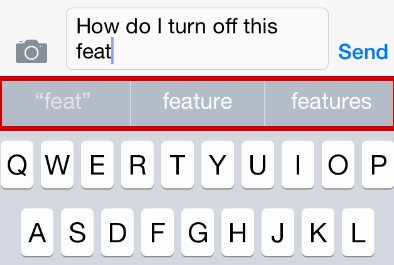
\includegraphics{predictive_keyboard}
        \caption{Fundamentally LLMs like GPT-3 (which drives ChatGPT) are using the same techniques as a predictive keyboard on your phone. This is why Yann Lecun says they are not particularly innovative. \url{https://www.youtube.com/watch?v=ULbpPHjiSBg}}
        \labfig{predictivekey}
\end{marginfigure}

Many models work like magic and many users assume models are predicting the future, when they are really correlating based on their past data. Even simple models of creditworthiness might have as similar problem. While building a creditworthiness model for a bank, due to lack of data a machine learning engineer might \sidenote{On purpose or inadvertently. }create a model that predicts whether someone is a smoker instead of whether they are creditworthy. Because smoking and poverty are correlated, maybe the model "works", but it doesn't do what stakeholders think it does. 

Setting expectations is another hellscape of misaligned incentives.\sidenote{The CEO of OpenAI wrote this and still raised ten billion dollars: \textit{"ChatGPT is incredibly limited, but good enough at some things to create a misleading impression of greatness. it's a mistake to be relying on it for anything important right now. it’s a preview of progress; we have lots of work to do on robustness and truthfulness."} \url{https://twitter.com/sama/status/1601731295792414720}} Good machine learning engineers and data scientists are supposed to educate and advise stakeholders about the limitations of their own models. Read Chollet's advice on this topic below:

\textit{The expectations of non-specialists towards AI systems are often unrealistic. For example, they might expect that the system “understands” its task and is capable of exercising human-like common sense in the context of the task. To address this, you should consider showing some examples of the failure modes of your model (for instance, show what incorrectly classified samples look like, especially those for which the misclassification seems surprising).} 

\textit{They might also expect human-level performance, especially for processes that were previously handled by people. Most machine learning models, because they are (imperfectly) trained to approximate human-generated labels, do not nearly get there. You should clearly convey model performance expectations. Avoid using abstract statements like “The model has 98 percent accuracy” (which most people mentally round up to 100 percent), and prefer talking, for instance, about false negative rates and false positive rates. You could say, “With these settings, the fraud detection model would have a 5 percent false negative rate and a 2.5 percent false positive rate. Every day, an average of 200 valid transactions would be flagged as fraudulent and sent for manual review, and an average of 14 fraudulent transactions would be missed. An average of 266 fraudulent transactions would be correctly caught.” Clearly relate the model’s performance metrics to business goals.}


\textit{You should also make sure to discuss with stakeholders the choice of key launch parameters—for instance, the probability threshold at which a transaction should be flagged (different thresholds will produce different false negative and false positive rates). Such decisions involve trade-offs that can only be handled with a deep understanding of the business context.}\cite{chollet2022} 

One does not need to be a psychologist to understand that these conversations almost never happen. The workflow of machine learning is universal, we are all doing fancy regressions and we all deal with the same wild expectations, shitty data and misalignment with business.

\begin{marginfigure}[-5.5cm]
        
\includegraphics{sciencechat}
        \caption{"mdjrny-v4 a handsome businessperson explaining the business context to a scientist wearing a white coat over coffee 8k" made with OpenJourney}
        \labfig{sciencechat}
\end{marginfigure}


\section{Key Takeaways}

\begin{itemize}
    \item \textbf{Deep learning models are fundamentally large unscientific regressions} they are trained to create a function that maps input data to output data.
    \item \textbf{Deep learning models are chaotic systems containing millions of interacting parameters} they are not designed to be explained or created in a way that their weights can be used for scientific analysis. They find reasonable answers and don't care how they get there. Multicolinearity (understanding the relationship of an input and output) and feature importance (understanding which inputs are most important) are only understandable with a high level of statistical error.
    \item \textbf{Small changes in inputs of a deep learning model may dramatically change the outputs} deep learning models are complex deterministic systems that can exhibit chaotic behavior. Their inner workings are functionally unknowable and practically impossible to test.
    \item \textbf{Deep learning models can have impressive and useful outputs, but the creators of models should be encouraged to highlight their failures and limitations.} Machine learning engineers might be more keen to highlight failures and limitations if they are encouraged to do so by their users, managers and investors.
\end{itemize}

